% Options for packages loaded elsewhere
\PassOptionsToPackage{unicode}{hyperref}
\PassOptionsToPackage{hyphens}{url}
\PassOptionsToPackage{dvipsnames,svgnames,x11names}{xcolor}
%
\documentclass[
  letterpaper,
  DIV=11,
  numbers=noendperiod]{scrartcl}

\usepackage{amsmath,amssymb}
\usepackage{iftex}
\ifPDFTeX
  \usepackage[T1]{fontenc}
  \usepackage[utf8]{inputenc}
  \usepackage{textcomp} % provide euro and other symbols
\else % if luatex or xetex
  \usepackage{unicode-math}
  \defaultfontfeatures{Scale=MatchLowercase}
  \defaultfontfeatures[\rmfamily]{Ligatures=TeX,Scale=1}
\fi
\usepackage{lmodern}
\ifPDFTeX\else  
    % xetex/luatex font selection
\fi
% Use upquote if available, for straight quotes in verbatim environments
\IfFileExists{upquote.sty}{\usepackage{upquote}}{}
\IfFileExists{microtype.sty}{% use microtype if available
  \usepackage[]{microtype}
  \UseMicrotypeSet[protrusion]{basicmath} % disable protrusion for tt fonts
}{}
\makeatletter
\@ifundefined{KOMAClassName}{% if non-KOMA class
  \IfFileExists{parskip.sty}{%
    \usepackage{parskip}
  }{% else
    \setlength{\parindent}{0pt}
    \setlength{\parskip}{6pt plus 2pt minus 1pt}}
}{% if KOMA class
  \KOMAoptions{parskip=half}}
\makeatother
\usepackage{xcolor}
\setlength{\emergencystretch}{3em} % prevent overfull lines
\setcounter{secnumdepth}{-\maxdimen} % remove section numbering
% Make \paragraph and \subparagraph free-standing
\ifx\paragraph\undefined\else
  \let\oldparagraph\paragraph
  \renewcommand{\paragraph}[1]{\oldparagraph{#1}\mbox{}}
\fi
\ifx\subparagraph\undefined\else
  \let\oldsubparagraph\subparagraph
  \renewcommand{\subparagraph}[1]{\oldsubparagraph{#1}\mbox{}}
\fi


\providecommand{\tightlist}{%
  \setlength{\itemsep}{0pt}\setlength{\parskip}{0pt}}\usepackage{longtable,booktabs,array}
\usepackage{calc} % for calculating minipage widths
% Correct order of tables after \paragraph or \subparagraph
\usepackage{etoolbox}
\makeatletter
\patchcmd\longtable{\par}{\if@noskipsec\mbox{}\fi\par}{}{}
\makeatother
% Allow footnotes in longtable head/foot
\IfFileExists{footnotehyper.sty}{\usepackage{footnotehyper}}{\usepackage{footnote}}
\makesavenoteenv{longtable}
\usepackage{graphicx}
\makeatletter
\def\maxwidth{\ifdim\Gin@nat@width>\linewidth\linewidth\else\Gin@nat@width\fi}
\def\maxheight{\ifdim\Gin@nat@height>\textheight\textheight\else\Gin@nat@height\fi}
\makeatother
% Scale images if necessary, so that they will not overflow the page
% margins by default, and it is still possible to overwrite the defaults
% using explicit options in \includegraphics[width, height, ...]{}
\setkeys{Gin}{width=\maxwidth,height=\maxheight,keepaspectratio}
% Set default figure placement to htbp
\makeatletter
\def\fps@figure{htbp}
\makeatother

\KOMAoption{captions}{tableheading}
\makeatletter
\@ifpackageloaded{tcolorbox}{}{\usepackage[skins,breakable]{tcolorbox}}
\@ifpackageloaded{fontawesome5}{}{\usepackage{fontawesome5}}
\definecolor{quarto-callout-color}{HTML}{909090}
\definecolor{quarto-callout-note-color}{HTML}{0758E5}
\definecolor{quarto-callout-important-color}{HTML}{CC1914}
\definecolor{quarto-callout-warning-color}{HTML}{EB9113}
\definecolor{quarto-callout-tip-color}{HTML}{00A047}
\definecolor{quarto-callout-caution-color}{HTML}{FC5300}
\definecolor{quarto-callout-color-frame}{HTML}{acacac}
\definecolor{quarto-callout-note-color-frame}{HTML}{4582ec}
\definecolor{quarto-callout-important-color-frame}{HTML}{d9534f}
\definecolor{quarto-callout-warning-color-frame}{HTML}{f0ad4e}
\definecolor{quarto-callout-tip-color-frame}{HTML}{02b875}
\definecolor{quarto-callout-caution-color-frame}{HTML}{fd7e14}
\makeatother
\makeatletter
\makeatother
\makeatletter
\makeatother
\makeatletter
\@ifpackageloaded{caption}{}{\usepackage{caption}}
\AtBeginDocument{%
\ifdefined\contentsname
  \renewcommand*\contentsname{Table of contents}
\else
  \newcommand\contentsname{Table of contents}
\fi
\ifdefined\listfigurename
  \renewcommand*\listfigurename{List of Figures}
\else
  \newcommand\listfigurename{List of Figures}
\fi
\ifdefined\listtablename
  \renewcommand*\listtablename{List of Tables}
\else
  \newcommand\listtablename{List of Tables}
\fi
\ifdefined\figurename
  \renewcommand*\figurename{Figure}
\else
  \newcommand\figurename{Figure}
\fi
\ifdefined\tablename
  \renewcommand*\tablename{Table}
\else
  \newcommand\tablename{Table}
\fi
}
\@ifpackageloaded{float}{}{\usepackage{float}}
\floatstyle{ruled}
\@ifundefined{c@chapter}{\newfloat{codelisting}{h}{lop}}{\newfloat{codelisting}{h}{lop}[chapter]}
\floatname{codelisting}{Listing}
\newcommand*\listoflistings{\listof{codelisting}{List of Listings}}
\makeatother
\makeatletter
\@ifpackageloaded{caption}{}{\usepackage{caption}}
\@ifpackageloaded{subcaption}{}{\usepackage{subcaption}}
\makeatother
\makeatletter
\@ifpackageloaded{tcolorbox}{}{\usepackage[skins,breakable]{tcolorbox}}
\makeatother
\makeatletter
\@ifundefined{shadecolor}{\definecolor{shadecolor}{rgb}{.97, .97, .97}}
\makeatother
\makeatletter
\makeatother
\makeatletter
\makeatother
\ifLuaTeX
  \usepackage{selnolig}  % disable illegal ligatures
\fi
\IfFileExists{bookmark.sty}{\usepackage{bookmark}}{\usepackage{hyperref}}
\IfFileExists{xurl.sty}{\usepackage{xurl}}{} % add URL line breaks if available
\urlstyle{same} % disable monospaced font for URLs
\hypersetup{
  pdftitle={Student Thesis: On-Boarding Checklist},
  pdfauthor={Alexander Smolka},
  colorlinks=true,
  linkcolor={blue},
  filecolor={Maroon},
  citecolor={Blue},
  urlcolor={Blue},
  pdfcreator={LaTeX via pandoc}}

\title{Student Thesis: On-Boarding Checklist}
\author{Alexander Smolka}
\date{2023-08-31}

\begin{document}
\maketitle
\ifdefined\Shaded\renewenvironment{Shaded}{\begin{tcolorbox}[borderline west={3pt}{0pt}{shadecolor}, frame hidden, boxrule=0pt, sharp corners, interior hidden, enhanced, breakable]}{\end{tcolorbox}}\fi

\begin{center}\rule{0.5\linewidth}{0.5pt}\end{center}

This page contains a checklist for students to get started working on
their thesis based on the \textbf{ExESS} research project. While the
\protect\hyperlink{sec-general}{General Checklist} is applicable to
students of all levels (Bachelor/Semester/Master) and all topics
(theoretical/numerical/\ldots); the other lists are only relevant for
certain levels and topics. For questions, please get in touch with me:
\href{mailto:a.smolka@tum.de}{\nolinkurl{a.smolka@tum.de}}.

\hypertarget{sec-general}{%
\subsection{General Checklist}\label{sec-general}}

This general checklist shall be completed in the first week(s) of your
student thesis work.

\begin{itemize}
\tightlist
\item[$\square$]
  receive ``LPE Thesis Starter Set''

  \begin{itemize}
  \tightlist
  \item
    read and understand the ``Student Thesis Information'' presentation
    slides
  \end{itemize}
\item[$\square$]
  open (and/or install) \href{https://matrix.tum.de/}{Matrix} and log in
  using your TUM-ID

  \begin{itemize}
  \tightlist
  \item
    use Matrix to send me a message containing one of the logical
    fallacies listed in the ``Student Thesis Information''
  \end{itemize}
\item[$\square$]
  set up \href{https://syncandshare.lrz.de/}{LRZ Sync\&Share} online
  folder
\item[$\square$]
  register your thesis

  \begin{itemize}
  \tightlist
  \item
    check the information on the registration document (LRZ Sync\&Share
    folder), sign the document, and upload the signed registration to
    the same folder
  \end{itemize}
\item[$\square$]
  set up a weekly meeting (including a fixed, weekly repeating outlook
  meeting)

  \begin{itemize}
  \tightlist
  \item
    please prepare a short presentation for each regular meeting, which
    should at a minimum, contain two slides: one with a list of the
    tasks you have completed since the last meeting and one with a list
    of the tasks you plan to complete until the next meeting
  \end{itemize}
\item[$\square$]
  set up a time plan for your thesis and include the plan in your first
  presentation (\emph{see the example below})
\end{itemize}

\begin{tcolorbox}[enhanced jigsaw, left=2mm, opacityback=0, title=\textcolor{quarto-callout-note-color}{\faInfo}\hspace{0.5em}{Example Time-Plan}, breakable, colback=white, toptitle=1mm, toprule=.15mm, colframe=quarto-callout-note-color-frame, bottomrule=.15mm, opacitybacktitle=0.6, bottomtitle=1mm, colbacktitle=quarto-callout-note-color!10!white, coltitle=black, titlerule=0mm, leftrule=.75mm, arc=.35mm, rightrule=.15mm]

The first time plan does not need to be (can not and should not be) very
detailed. It should, however, give a rough overview of the tasks you
plan to complete and the time you plan to spend on each task. The
following is an example of a first draft of a time plan for a 6-month
thesis. The time plan is written in
\href{https://mermaid-js.github.io/mermaid/\#/}{Mermaid}, which is a
markdown-like language for generating diagrams. The Mermaid code is
included in the source of this page, so you can copy it and modify it
for your own time-plan. You can also use the
\href{https://mermaid-js.github.io/mermaid-live-editor/}{Mermaid Live
Editor} to generate your own time plan.

For your thesis, revisit the time plan regularly and update it
accordingly. This will help you to keep track of your progress and to
identify potential problems early on. Adding more details to the time
plan over time will give you a good starting point for your thesis
report.

\begin{figure}[H]

{\centering 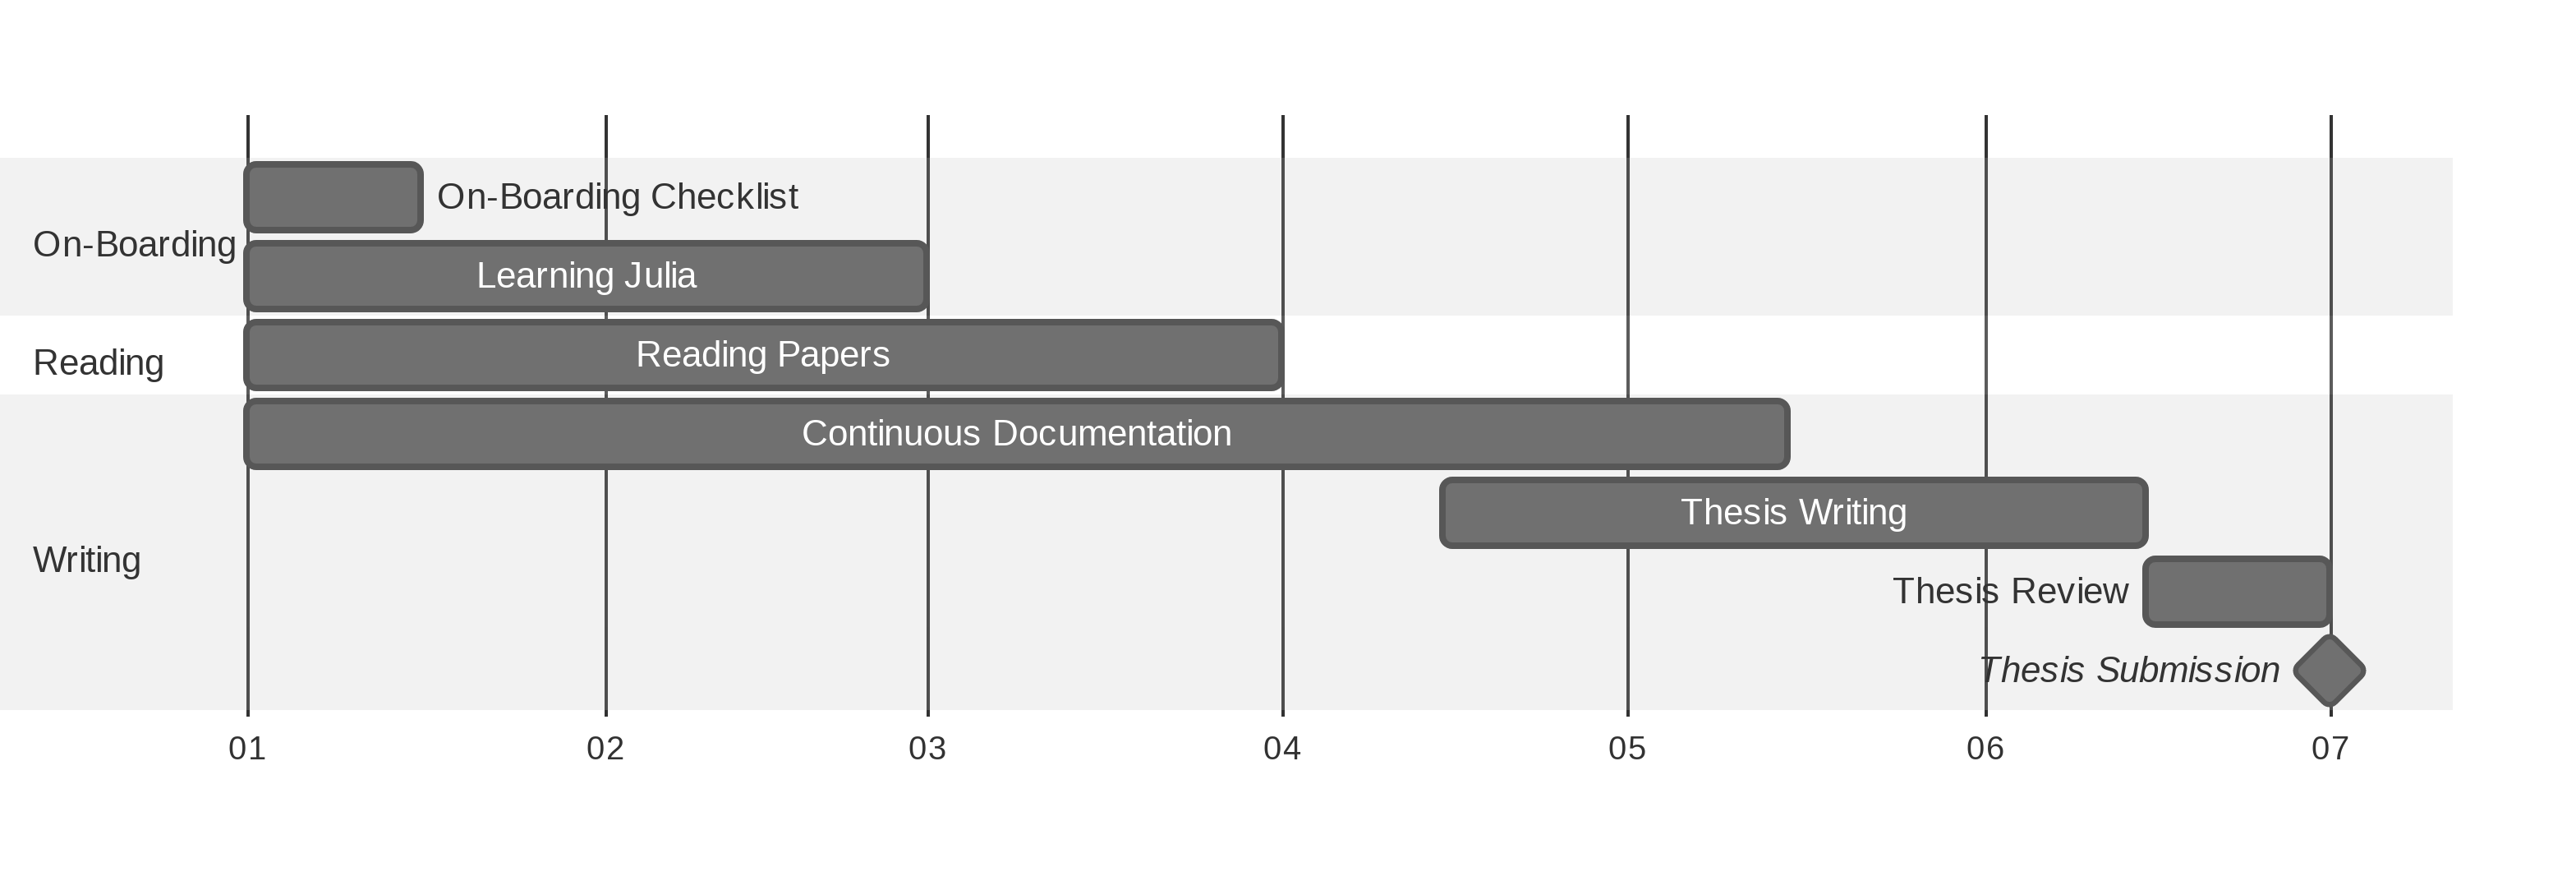
\includegraphics[width=6in,height=2.05in]{index_files/figure-latex/mermaid-figure-2.png}

}

\end{figure}

\end{tcolorbox}

\hypertarget{sec-numerical}{%
\subsection{Numerical Based Thesis Checklist}\label{sec-numerical}}

In case you are working on a numerical-based thesis, the following
checklist can help you get started with your work.

\begin{itemize}
\tightlist
\item[$\square$]
  set up \href{https://julialang.org/}{Julia}

  \begin{itemize}
  \tightlist
  \item
    check out the list with recommended
    \href{/manuals/julia_links/index.qmd}{Julia Resources}
  \end{itemize}
\item[$\square$]
  set up the \texttt{ExESS} package (if applicable)
\end{itemize}



\end{document}
